\documentclass[aspectratio=169]{beamer}
\mode<presentation>
\usetheme{Hannover}
\useoutertheme{sidebar}
\usecolortheme{dolphin}

\usepackage{amsmath}
\usepackage{amssymb}
\usepackage{enumerate}


% some bold math symbosl
\newcommand{\Cov}{\mathrm{Cov}}
\newcommand{\Cor}{\mathrm{Cor}}
\newcommand{\Var}{\mathrm{Var}}
\newcommand{\brho}{\boldsymbol{\rho}}
\newcommand{\bSigma}{\boldsymbol{\Sigma}}
\newcommand{\btheta}{\boldsymbol{\theta}}
\newcommand{\bbeta}{\boldsymbol{\beta}}
\newcommand{\bmu}{\boldsymbol{\mu}}
\newcommand{\bW}{\mathbf{W}}
\newcommand{\one}{\mathbf{1}}
\newcommand{\bH}{\mathbf{H}}
\newcommand{\by}{\mathbf{y}}
\newcommand{\bolde}{\mathbf{e}}
\newcommand{\bx}{\mathbf{x}}

\newcommand{\cpp}[1]{\texttt{#1}}

\title{Mathematical Biostatistics Boot Camp: Lecture 11, Plotting}
\author{Brian Caffo}
\date{\today}
\institute[Department of Biostatistics]{
  Department of Biostatistics \\
  Johns Hopkins Bloomberg School of Public Health\\
  Johns Hopkins University
}


\begin{document}

\frame{\titlepage}


\section{Table of contents}
\frame{
  \frametitle{Table of contents}
  \tableofcontents
}

\section{Histograms}
\begin{frame}\frametitle{Histograms}
\begin{itemize}
\item Histograms display a sample estimate of the density or mass
  function by plotting a bar graph of the frequency or proportion of
  times that a variable takes specific values, or a range of values
  for continuous data, within a sample
\end{itemize}
\end{frame}

\begin{frame}\frametitle{Example}
\begin{itemize}
\item The data set \texttt{islands} in the R package \texttt{datasets} contains
  the areas of all land masses in thousands of square miles
\item Load the data set with the command \texttt{data(islands)}
\item View the data by typing \texttt{islands}
\item Create a histogram with the command \texttt{hist(islands)}
\item Do \texttt{?hist} for options  
\end{itemize}
\end{frame}

\begin{frame}
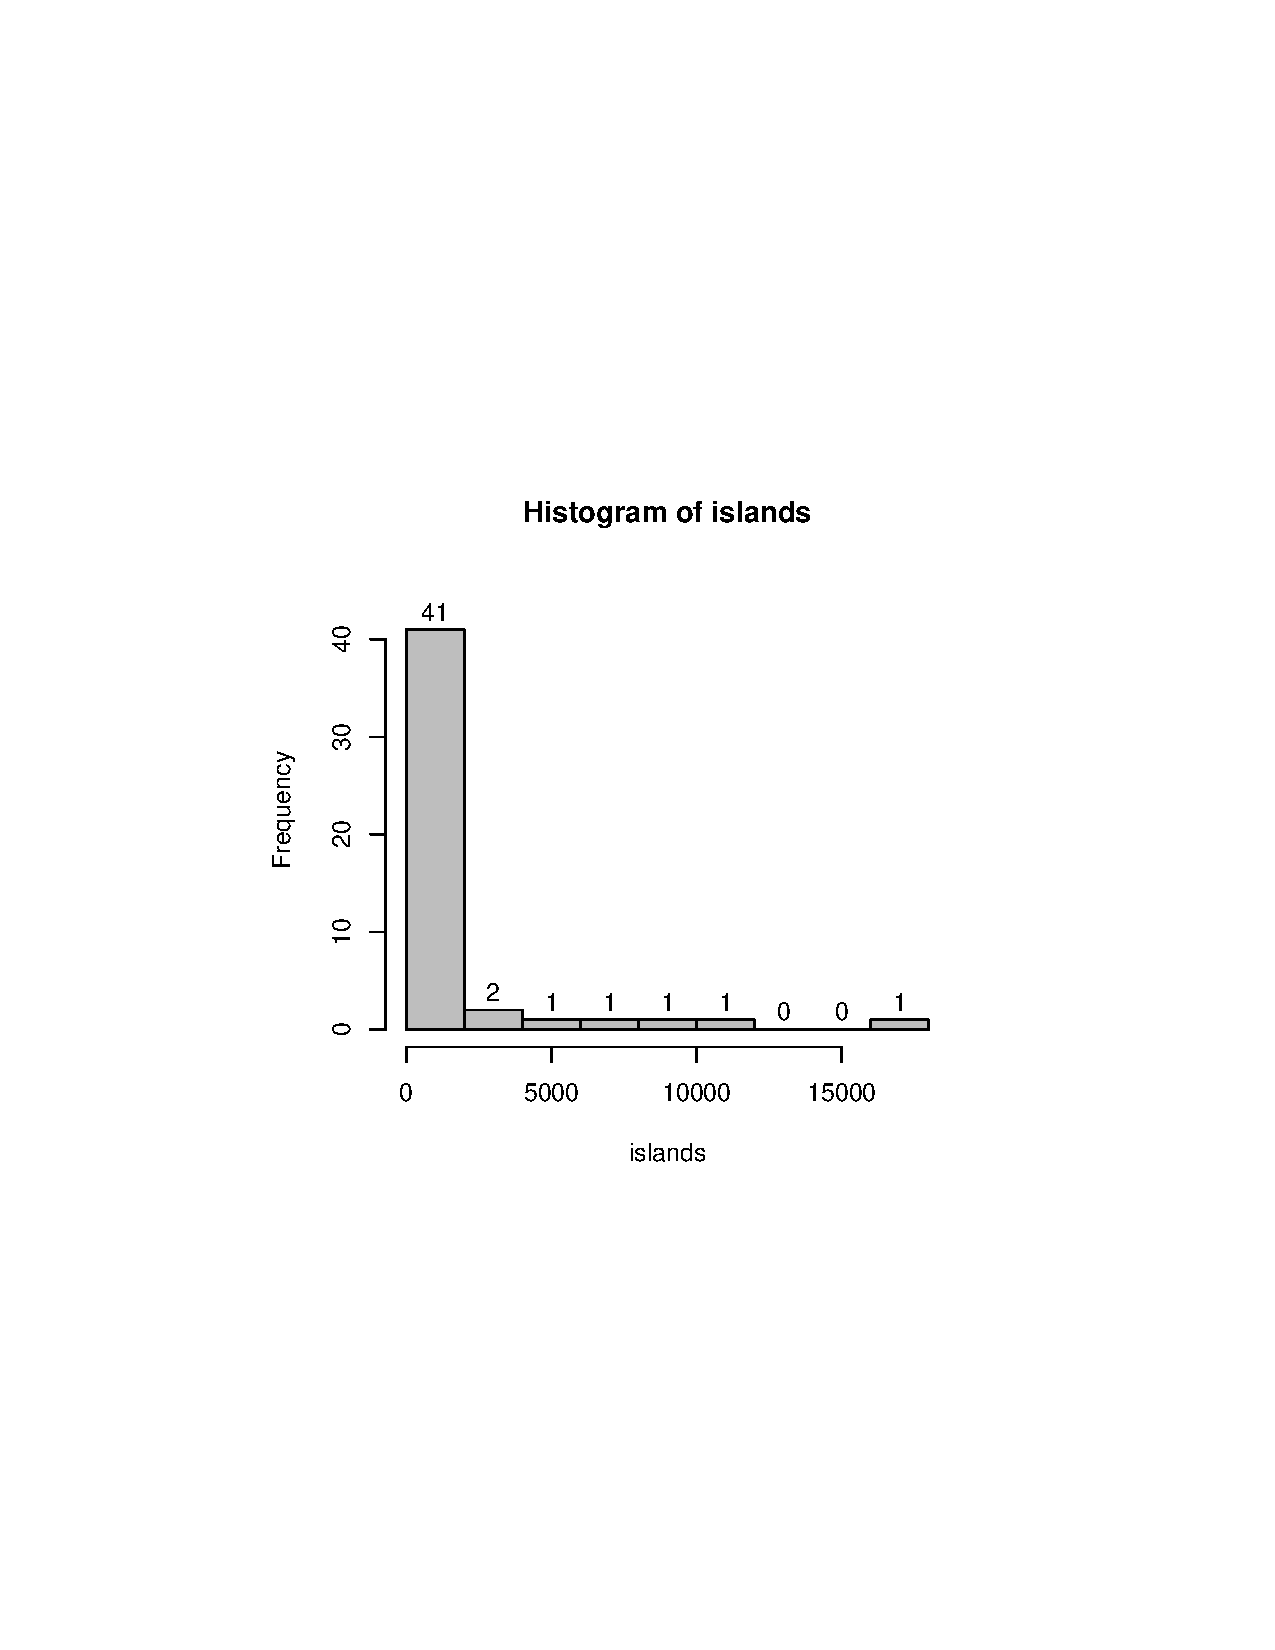
\includegraphics[width=3.5in]{hist.pdf}
\end{frame}

\begin{frame}\frametitle{Pros and cons}
\begin{itemize}
\item Histograms are useful and easy, apply to continuous, discrete and even
  unordered data
\item They use a lot of ink and space to display very little information
\item It's difficult to display several at the same time for comparisons
\end{itemize}
Also, for this data it's probably preferable to consider log base 10
(orders of magnitude), since the raw histogram simply says that most
islands are small 
\end{frame}


\begin{frame}
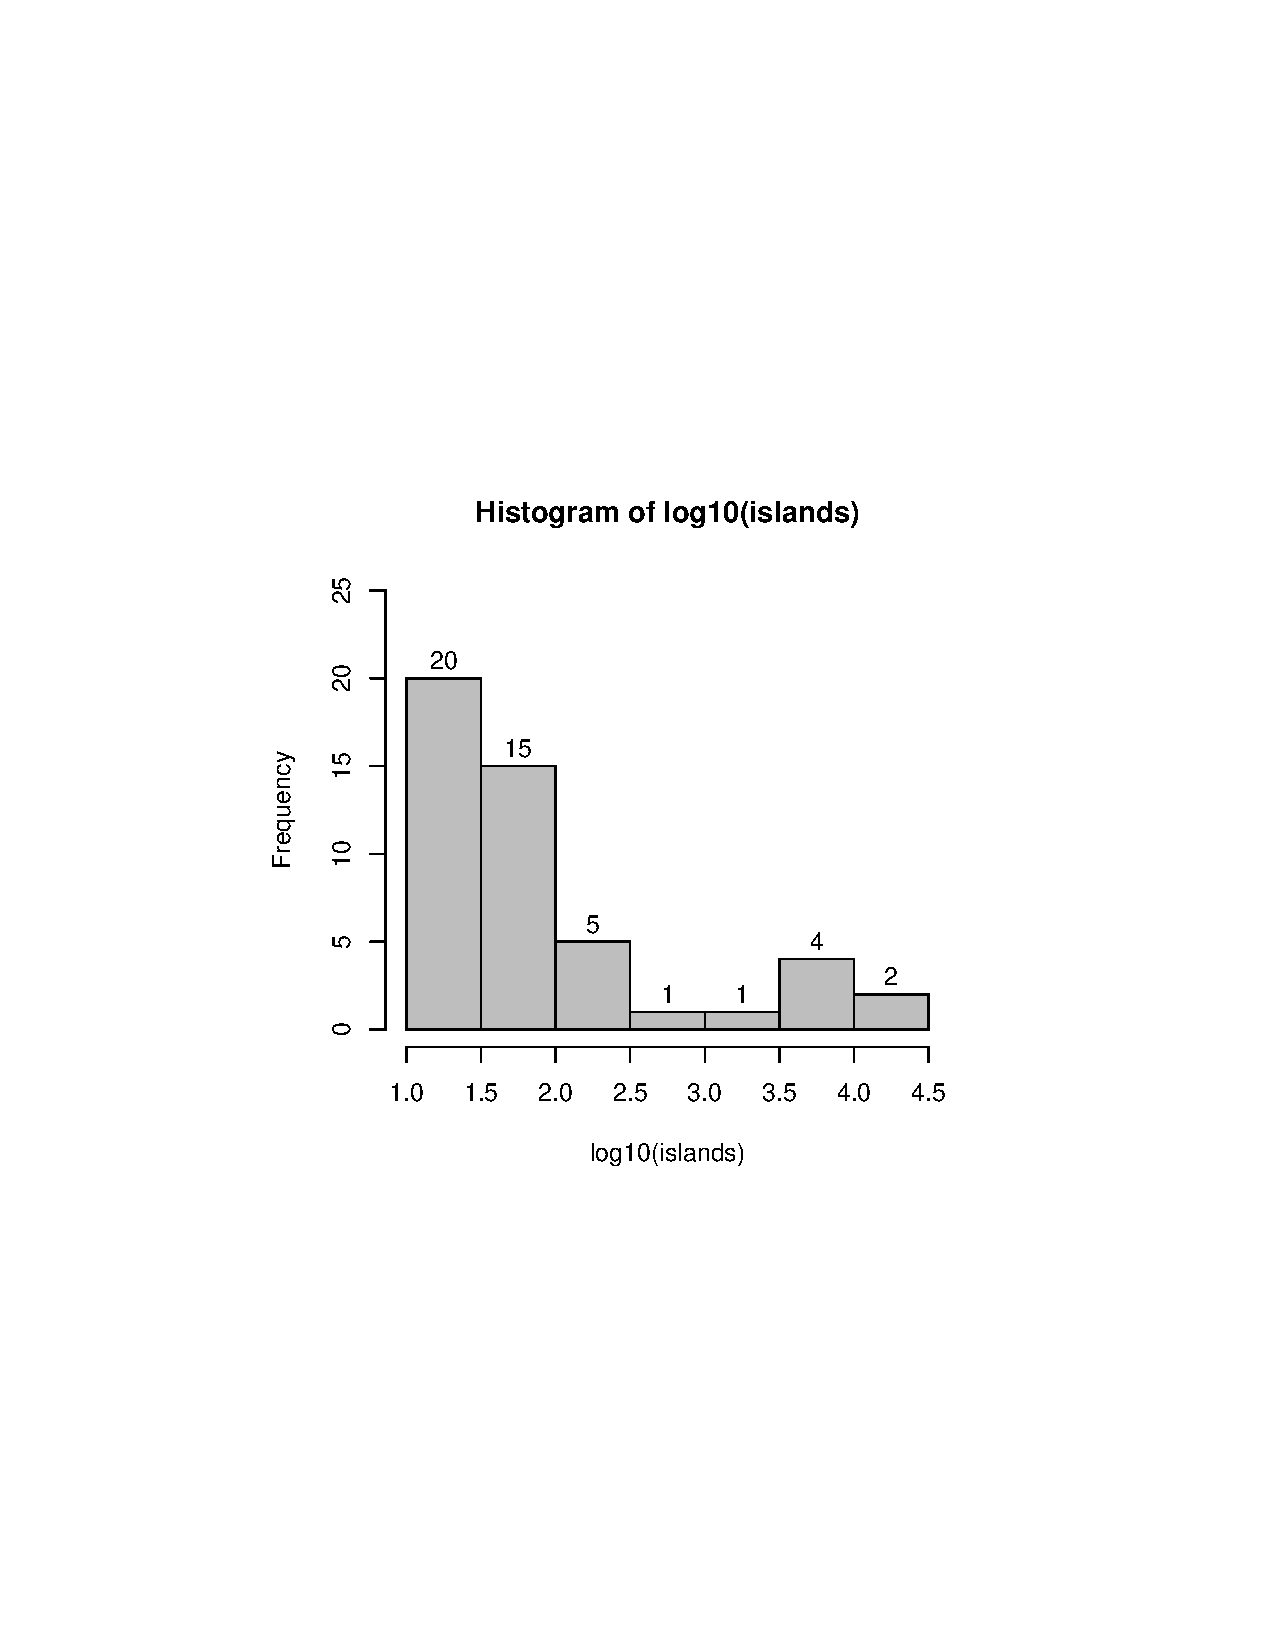
\includegraphics[width=3.5in]{histLog10.pdf}
\end{frame}

\section{Stem and leaf}
\begin{frame}\frametitle{Stem-and-leaf plots}
\begin{itemize}
\item Stem-and-leaf plots are extremely useful for getting
  distribution information on the fly
\item Read the text about creating them
\item They display the complete data set and so waste very little ink
\item Two data sets' stem and leaf plots can be shown back-to-back for
  comparisons
\item Created by John Tukey, a leading figure in the development of
  the statistical sciences and signal processing
\end{itemize}
\end{frame}

\begin{frame}[fragile]\frametitle{Example}
\begin{verbatim}
> stem(log10(islands))

  The decimal point is at the |

  1 | 1111112222233444
  1 | 5555556666667899999
  2 | 3344
  2 | 59
  3 | 
  3 | 5678
  4 | 012
\end{verbatim}
\end{frame}

\section{Dotcharts}
\begin{frame}\frametitle{Dotcharts}
\begin{itemize}
\item Dotcharts simply display a data set, one dot per point
\item Ordering of the dots and labeling of the axes
  can display additional information
\item Dotcharts show a complete data set and so have high
  data density
\item May be impossible to construct/difficult to interpret
  for data sets with lots of points
\end{itemize}
\end{frame}

\begin{frame}
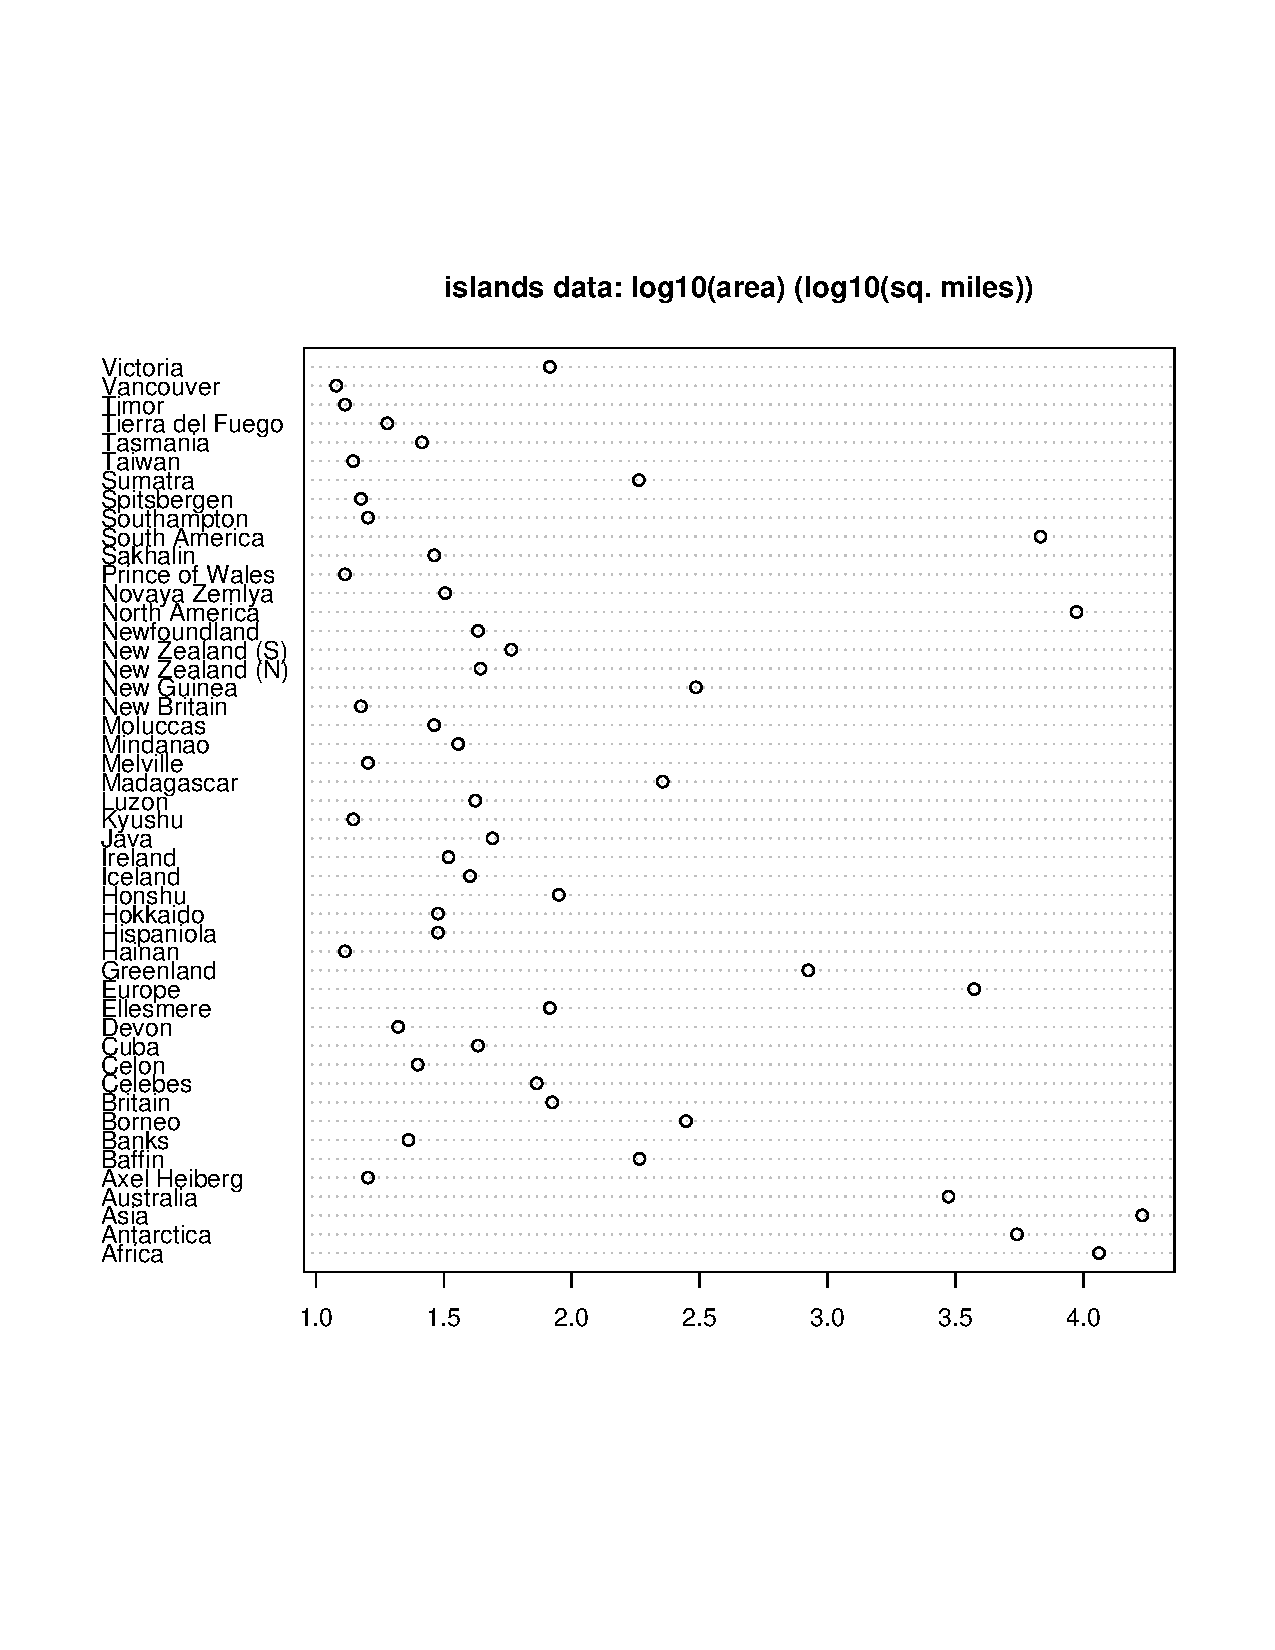
\includegraphics[width=3.5in]{dotChart.pdf}
\end{frame}

\begin{frame}\frametitle{Discussion}
\begin{itemize}
\item Maybe ordering alphabetically isn't the best thing for this data set
\item Perhaps grouped by continent, then nations by geography
  (grouping Pacific islands together)?
\end{itemize}
\end{frame}

\begin{frame}\frametitle{Dotplots comparing grouped data}
\begin{itemize}
\item For data sets in groups, you often want to display density
  information by group
\item If the size of the data permits, displaying the whole data
  is preferable
\item Add horizontal lines to depict means, medians
\item Add vertical lines to depict variation, show confidence intervals
  interquartile ranges
\item Jitter the points to avoid overplotting (\texttt{jitter})
\end{itemize}
\end{frame}

\begin{frame}[fragile]\frametitle{Example}
\begin{itemize}
\item The InsectSprays dataset contains counts of insect deaths by
  insecticide type (A, B, C, D, E, F)
\item You can obtain the data set with the command
\begin{verbatim}
data(InsectSprays)
\end{verbatim}
\end{itemize}
\end{frame}

\begin{frame}[fragile]
  The gist of the code is below
\begin{verbatim}
attach(InsectSprays)
plot(c(.5, 6.5), range(count))
sprayTypes <- unique(spray)
for (i in 1 : length(sprayTypes)){
  y <- count[spray == sprayTypes[i]]
  n <- sum(spray == sprayTypes[i])
  points(jitter(rep(i, n), amount = .1), y)
  lines(i + c(.12, .28), rep(mean(y), 2), lwd = 3)
  lines(rep(i + .2, 2), 
        mean(y) + c(-1.96, 1.96) * sd(y) / sqrt(n)
       )
}
\end{verbatim}
\end{frame}

\begin{frame}
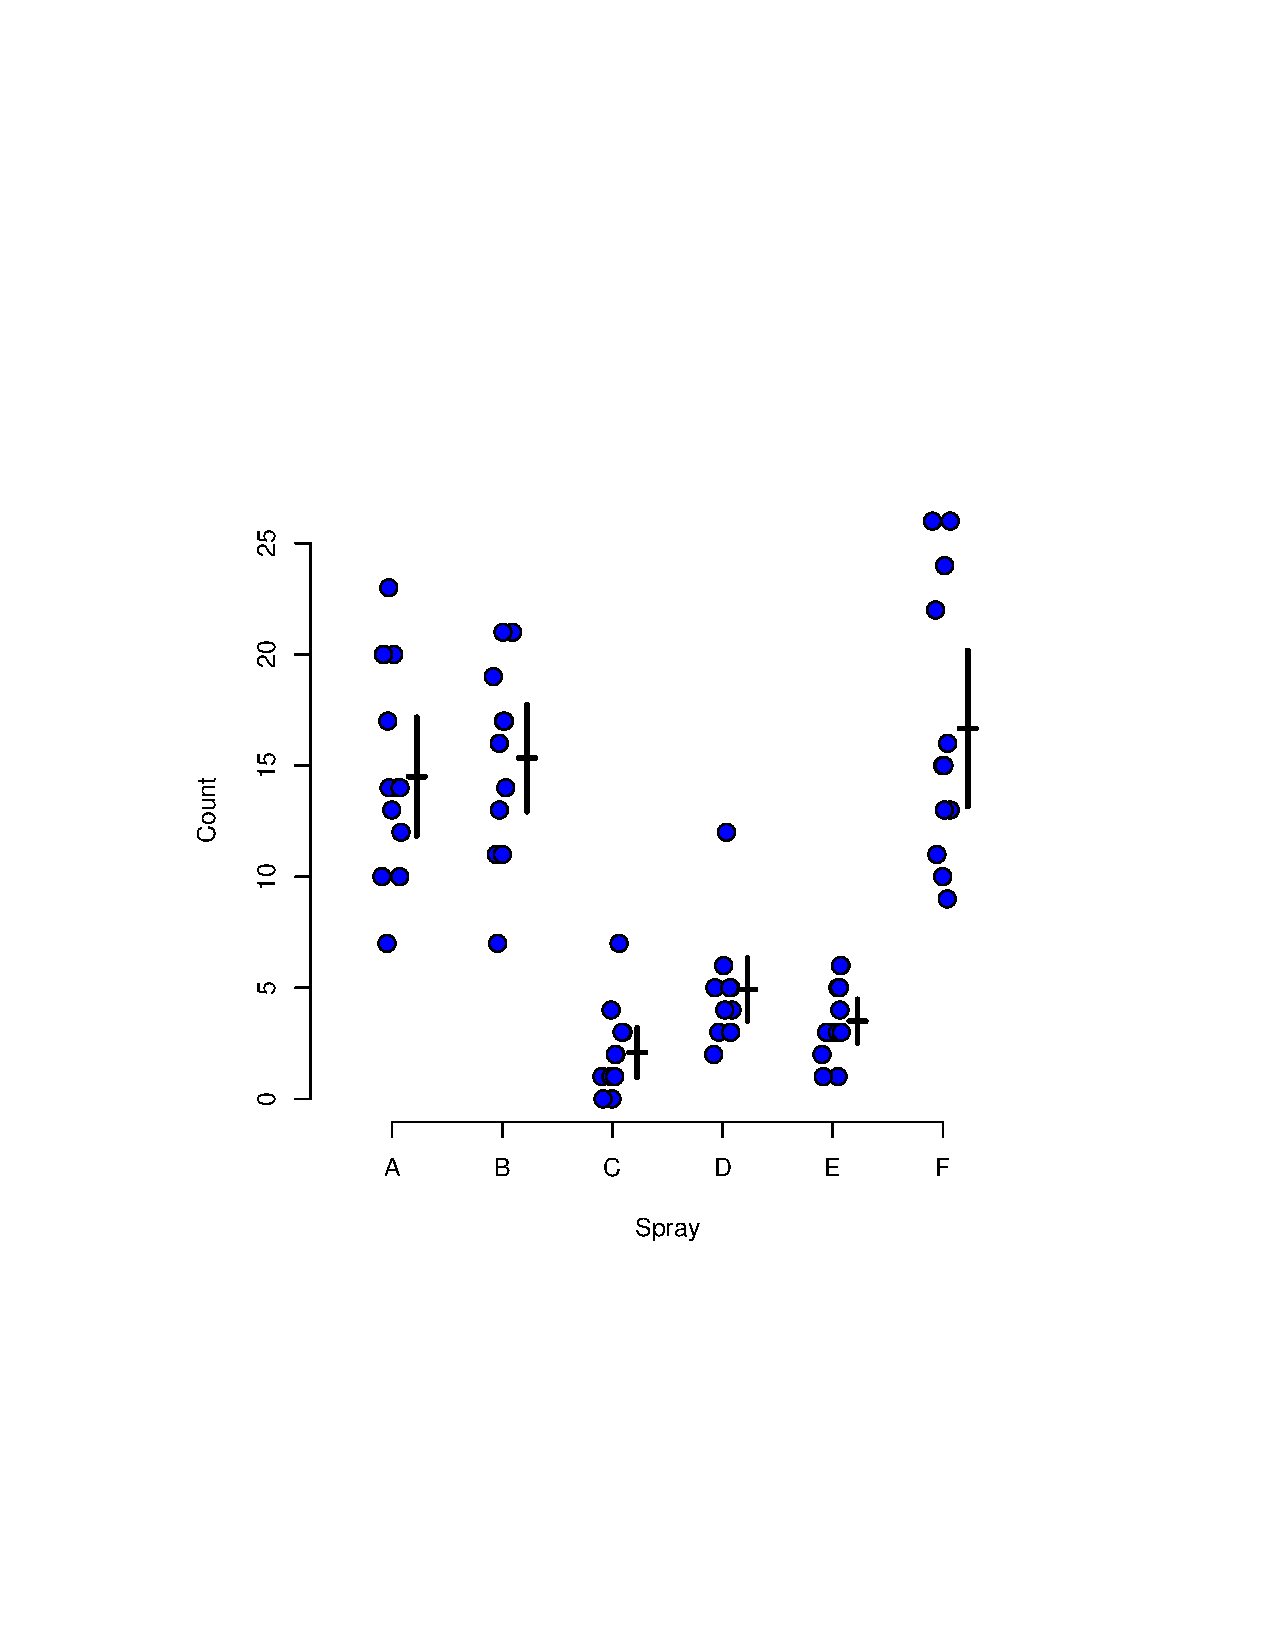
\includegraphics[width=3.5in]{dotPlot.pdf}
\end{frame}


\section{Boxplots}
\begin{frame}\frametitle{Boxplots}
\begin{itemize}
\item Boxplots are useful for the same sort of display as the dot
  chart, but in instances where displaying the whole data set is
  not possible
\item Centerline of the boxes represents the median while the 
  box edges correspond to the quartiles
\item Whiskers extend out to a constant times the IQR or the max value
\item Sometimes potential outliers are denoted by points beyond the whiskers
\item Also invented by Tukey
\item Skewness indicated by centerline being near one of the box edges
\end{itemize}
\end{frame}

\begin{frame}
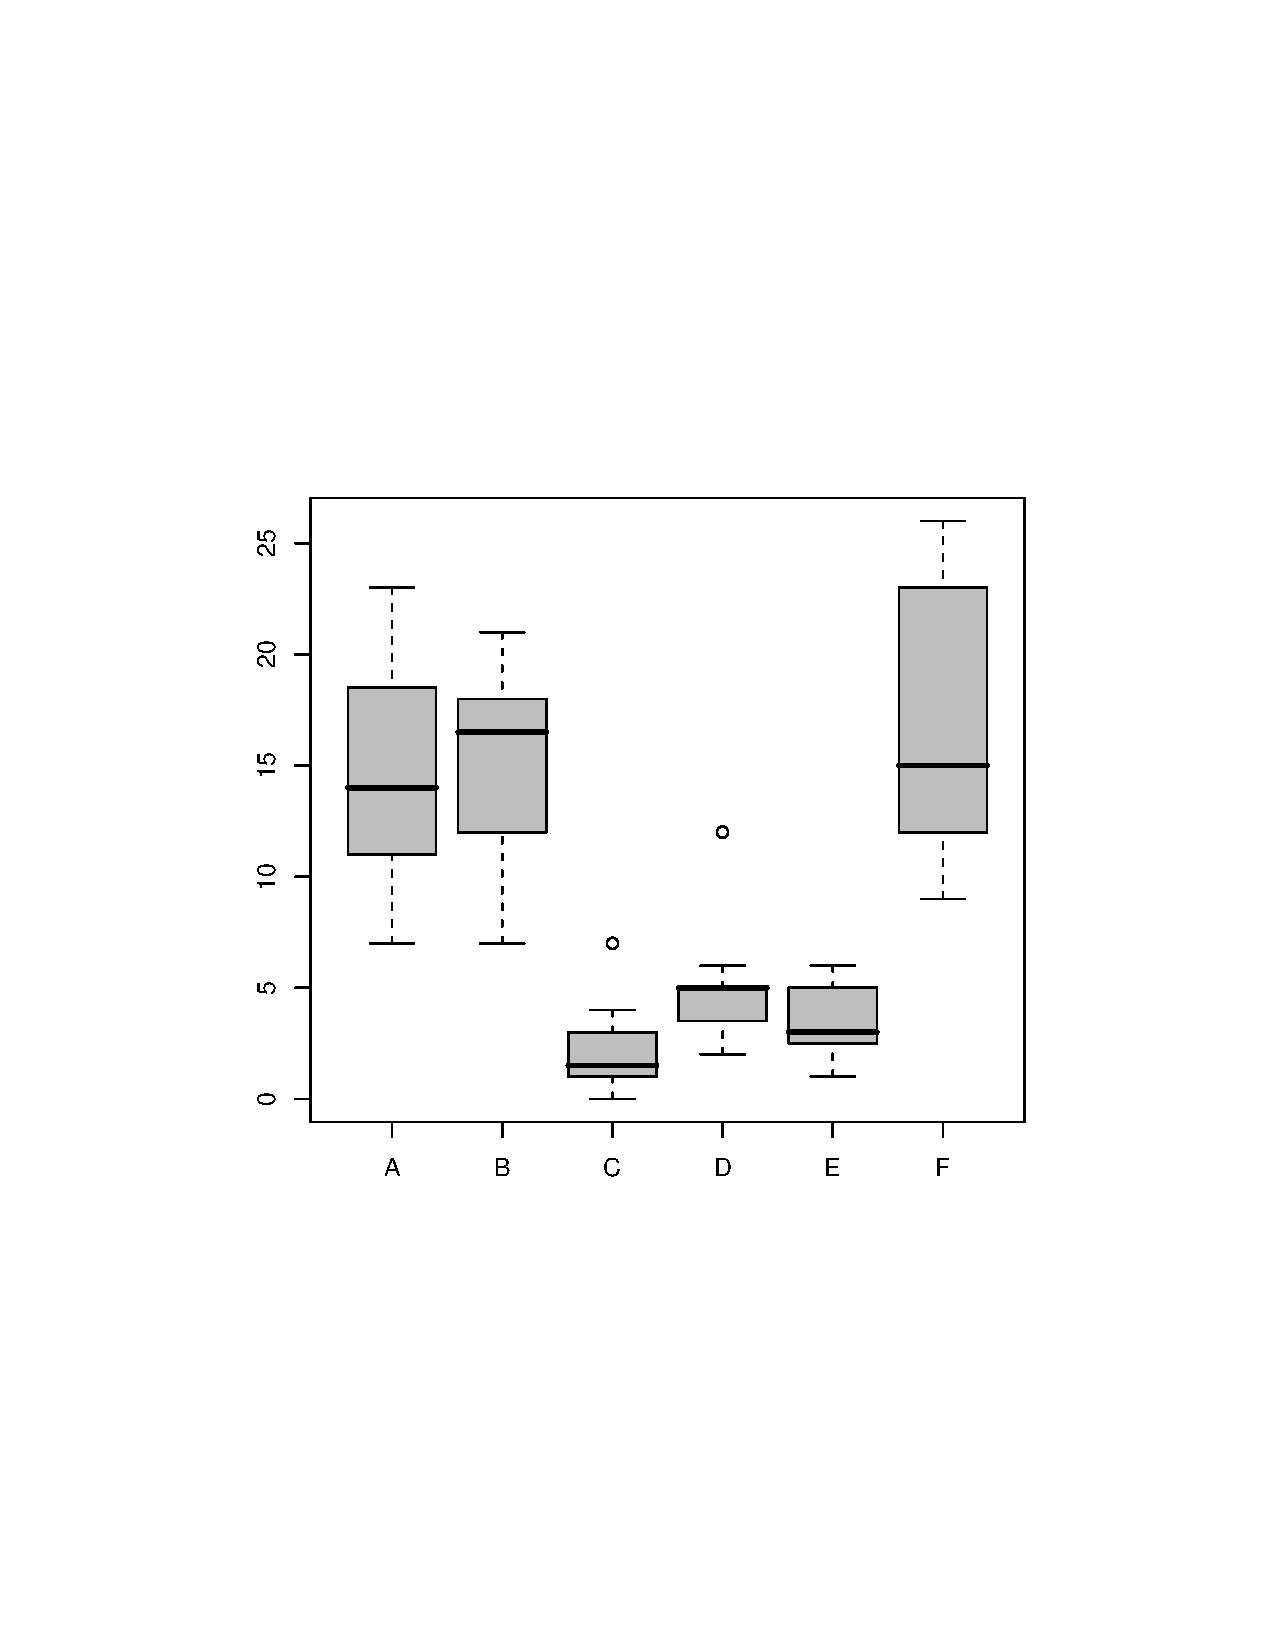
\includegraphics[width=3.5in]{boxplot.pdf}
\end{frame}

\begin{frame}[fragile]\frametitle{Boxplots discussion}
\begin{itemize}
\item Don't use boxplots for small numbers of observations, just plot the data!
\item Try logging if some of the boxes are too squished relative to other ones;
  you can convert the axis to unlogged units (though they will not be equally spaced
  anymore)
\item For data with lots and lots of observations omit the outliers
  plotting if you get so many of them that you can't see the points
\item Example of a bad box plot
\begin{verbatim}
boxplot(rt(500, 2))
\end{verbatim}
\end{itemize}
\end{frame}

\begin{frame}
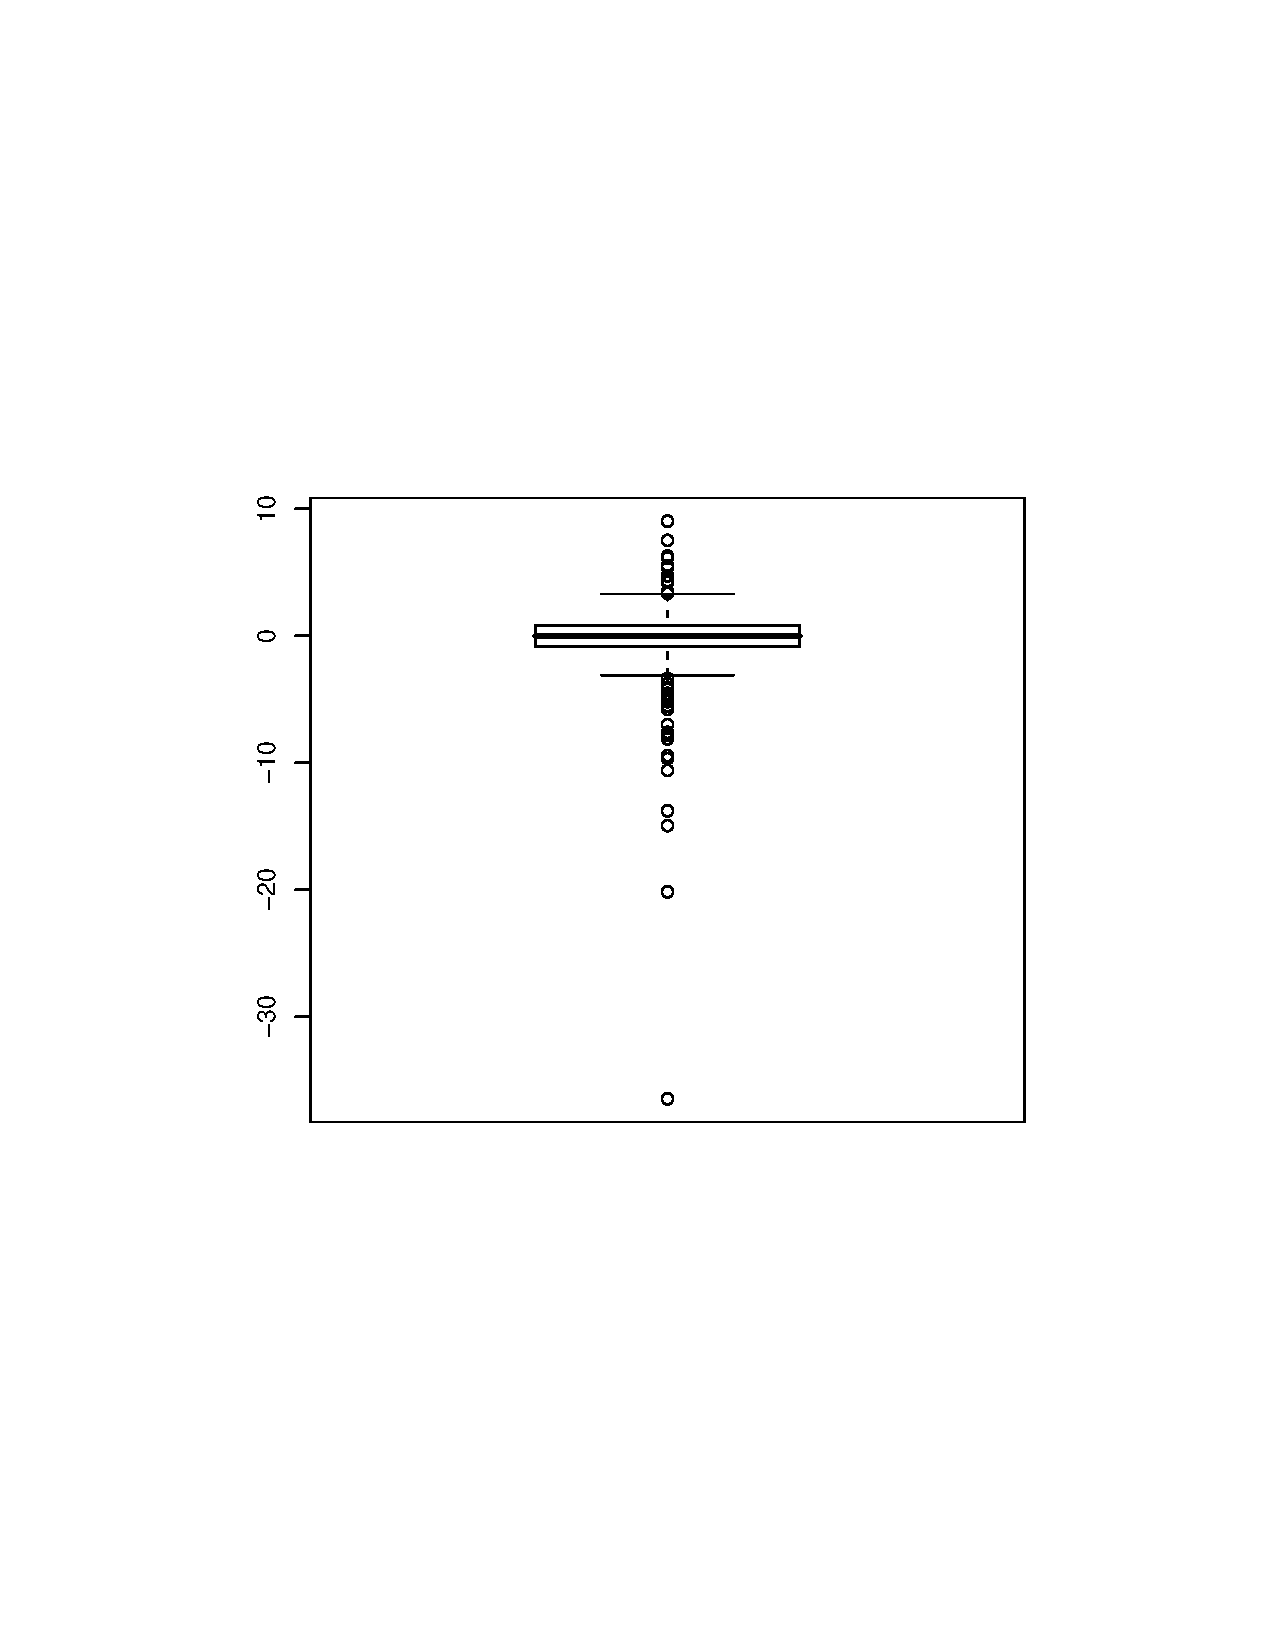
\includegraphics[width=3.5in]{boxplotBad.pdf}
\end{frame}

\section{KDEs}
\begin{frame}\frametitle{Kernel density estimates}
\begin{itemize}
\item Kernel density estimates are essentially more modern
  versions of histograms providing density estimates for
  continuous data
\item Observations are weighted according to a ``kernel'',
  in most cases a Gaussian density
\item ``Bandwidth'' of the kernel effectively plays the role of
  the bin size for the histogram
  \begin{enumerate}[a.]
  \item Too low of a bandwidth yields a too variable (jagged) measure
    of the density
  \item Too high of a bandwidth oversmooths
  \end{enumerate}
\item The R function \texttt{density} can be used to create KDEs
\end{itemize}
\end{frame}

\begin{frame}[fragile]\frametitle{Example} 
Data is the waiting and eruption times in minutes between
eruptions of the Old Faithful Geyser in Yellowstone National park
\begin{verbatim}
data(faithful)
d <- density(faithful$eruptions, bw = "sj")
plot(d)
\end{verbatim}
\end{frame}

\begin{frame}
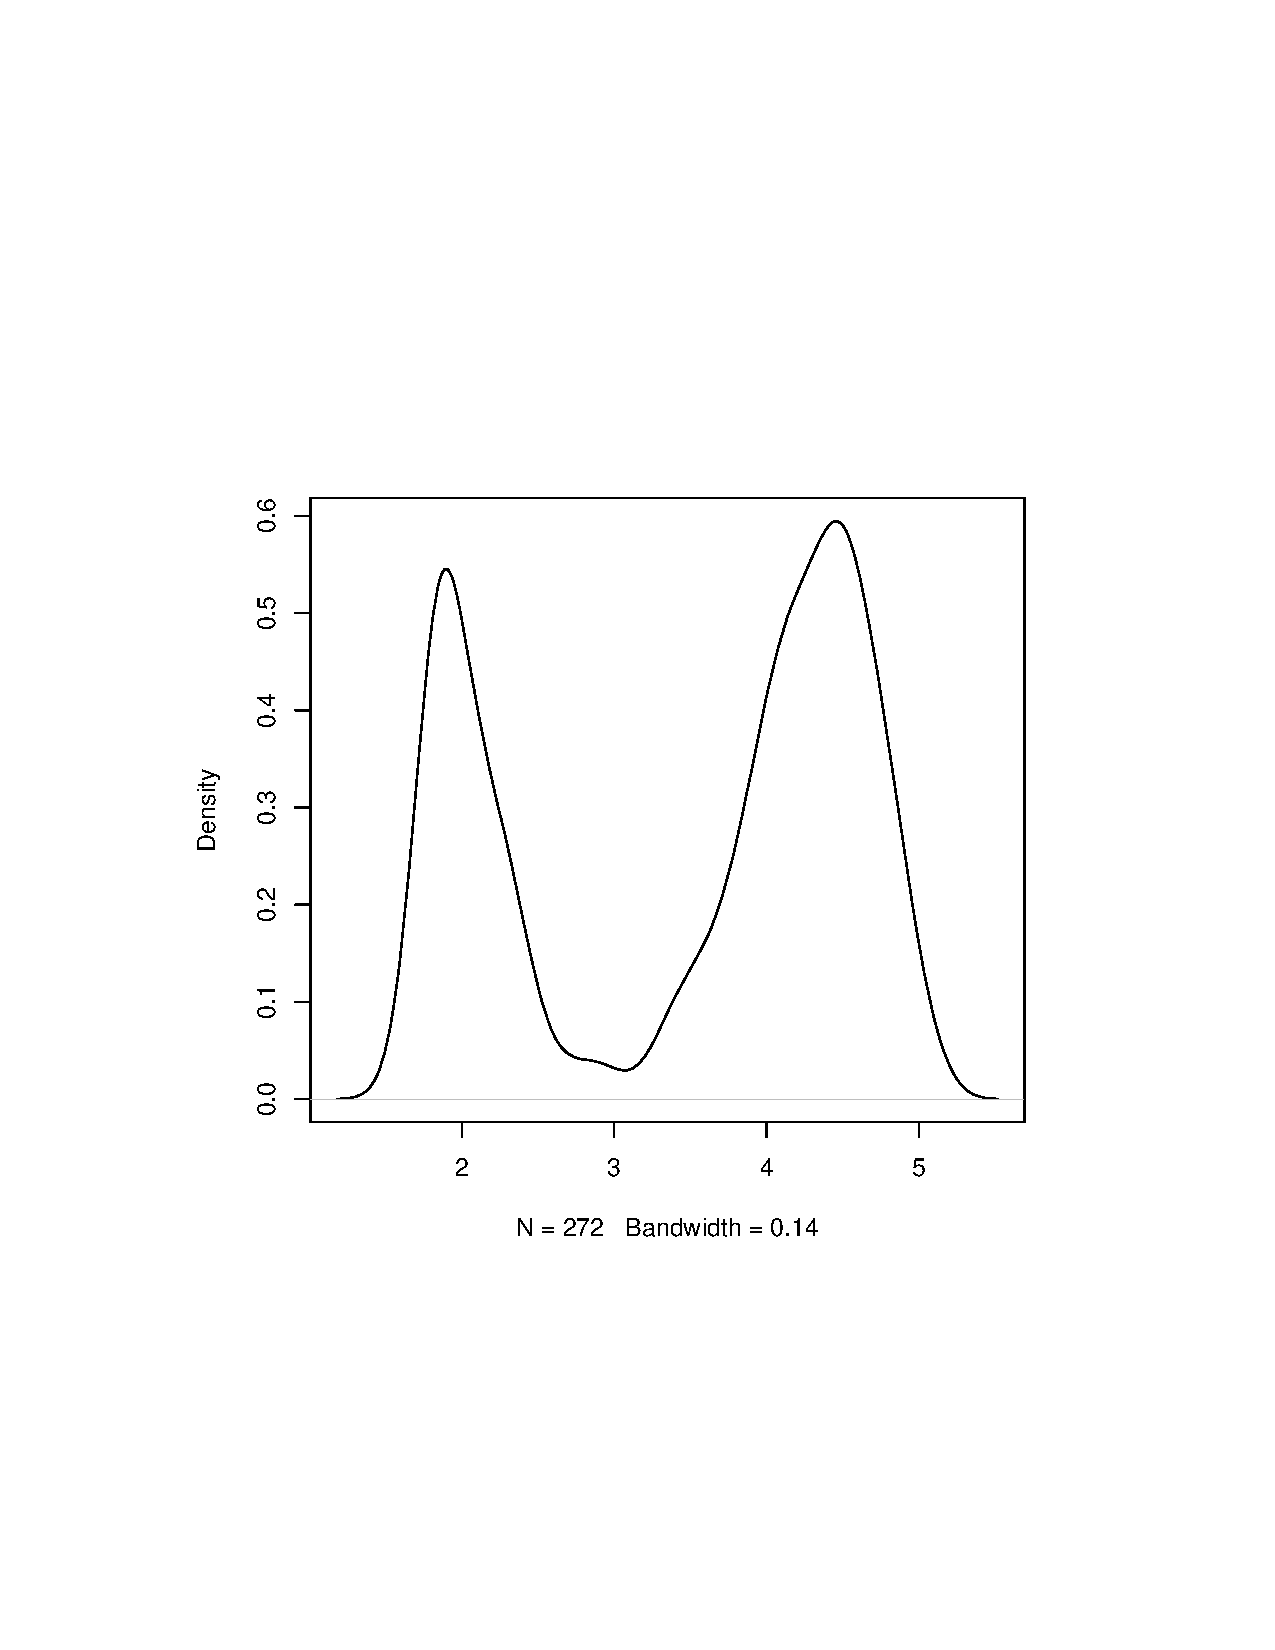
\includegraphics[width=3.5in]{kde.pdf}
\end{frame}

\begin{frame}\frametitle{Imaging example}
  \begin{itemize}
  \item Consider the following image slice (created in R) from a high resolution MRI of a brain
  \item This is a single (axial) slice of a three-dimensional image
  \item Consider discarding the location information and plotting a KDE of the intensities
  \end{itemize}
 \end{frame}

\begin{frame}
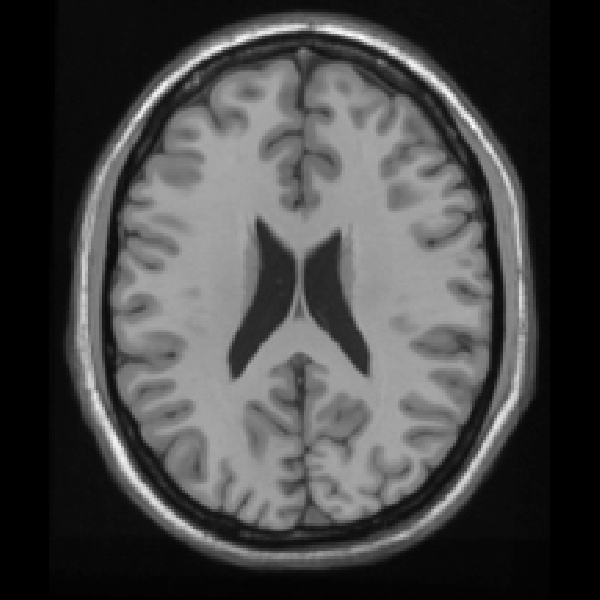
\includegraphics[width=3.5in]{brain.pdf}
\end{frame}

\begin{frame}
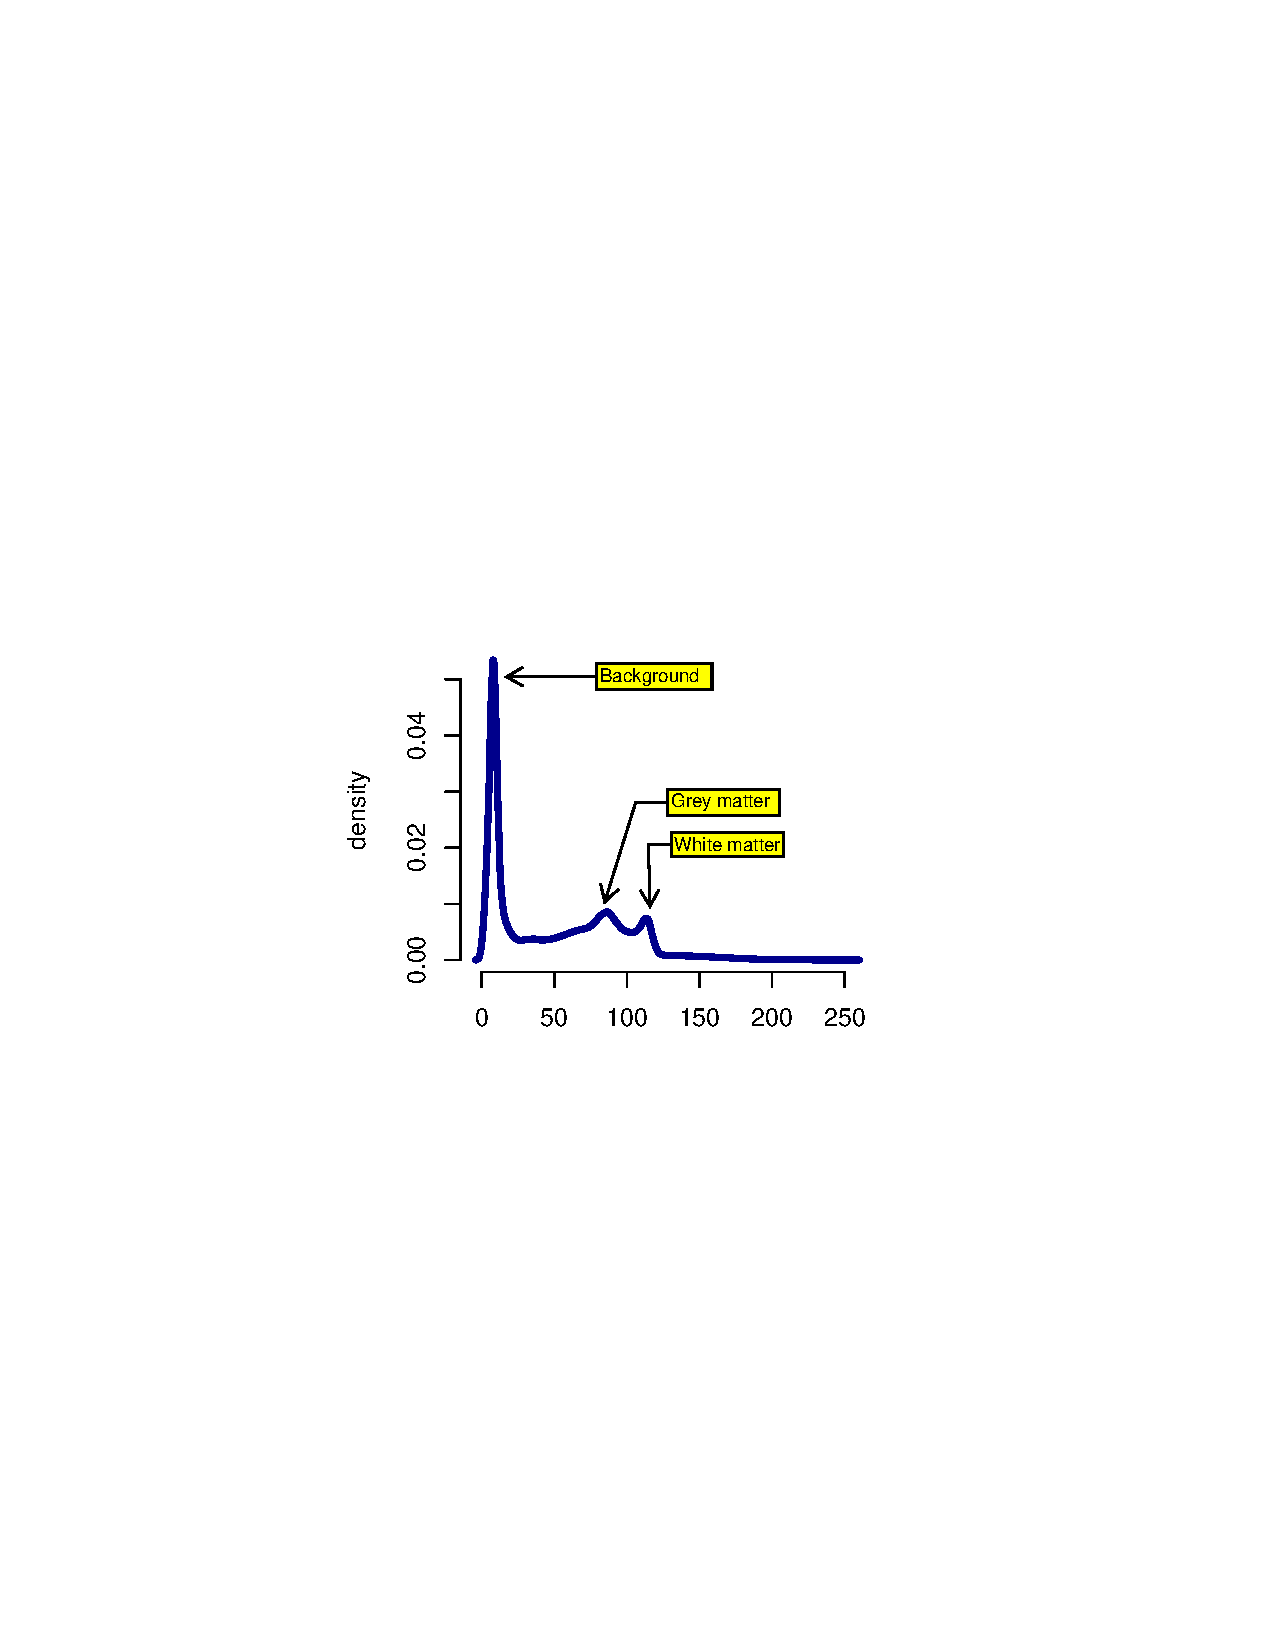
\includegraphics[width=3.5in]{brainDensityWithAnnotation.pdf}
\end{frame}

\section{QQ-plots}
\begin{frame}\frametitle{QQ-plots}
\begin{itemize}
\item QQ-plots (for quantile-quantile) are extremely useful
  for comparing data to a theoretical distribution
\item Plot the empirical quantiles against theoretical quantiles
\item Most useful for diagnosing normality
\end{itemize}
\end{frame}

\begin{frame}
\begin{itemize}
\item Let $x_p$ be the $p^{th}$ quantile from a $N(\mu, \sigma^2)$
\item Then $P(X \leq x_p) = p$
\item Clearly $P(Z \leq \frac{x_p - \mu}{\sigma}) = p$
\item Therefore $x_p = \mu + z_p \sigma$ (this should not be news)
\item Result, quantiles from a $N(\mu,\sigma^2)$ population should
  be linearly related to standard normal quantiles
\item A normal qq-plot plot the empirical quantiles against the
  theoretical standard normal quantiles
\item In R \texttt{qqnorm} for a normal QQ-plot and  \texttt{qqplot}
  for a qqplot against an arbitrary distribution
\end{itemize}
\end{frame}

\begin{frame}
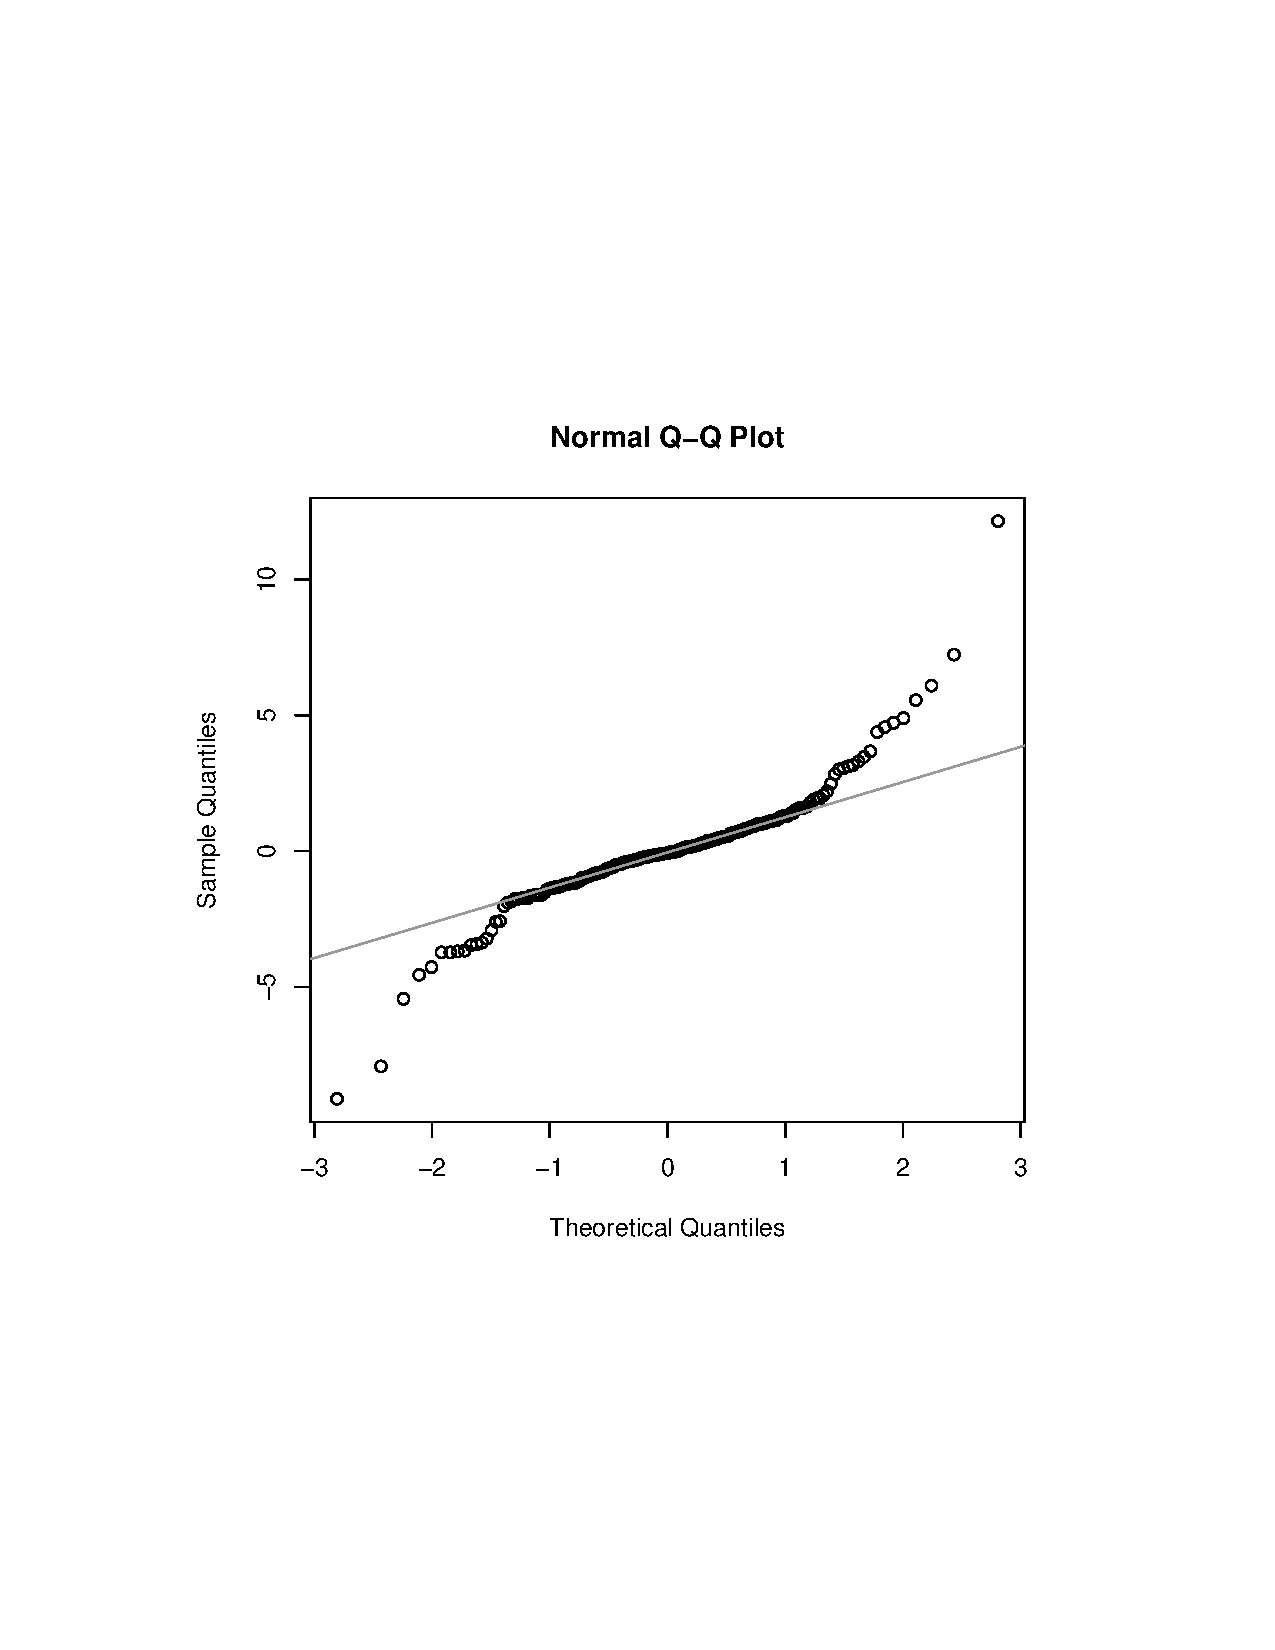
\includegraphics[width=3.5in]{qqnorm1.pdf}
\end{frame}

\begin{frame}
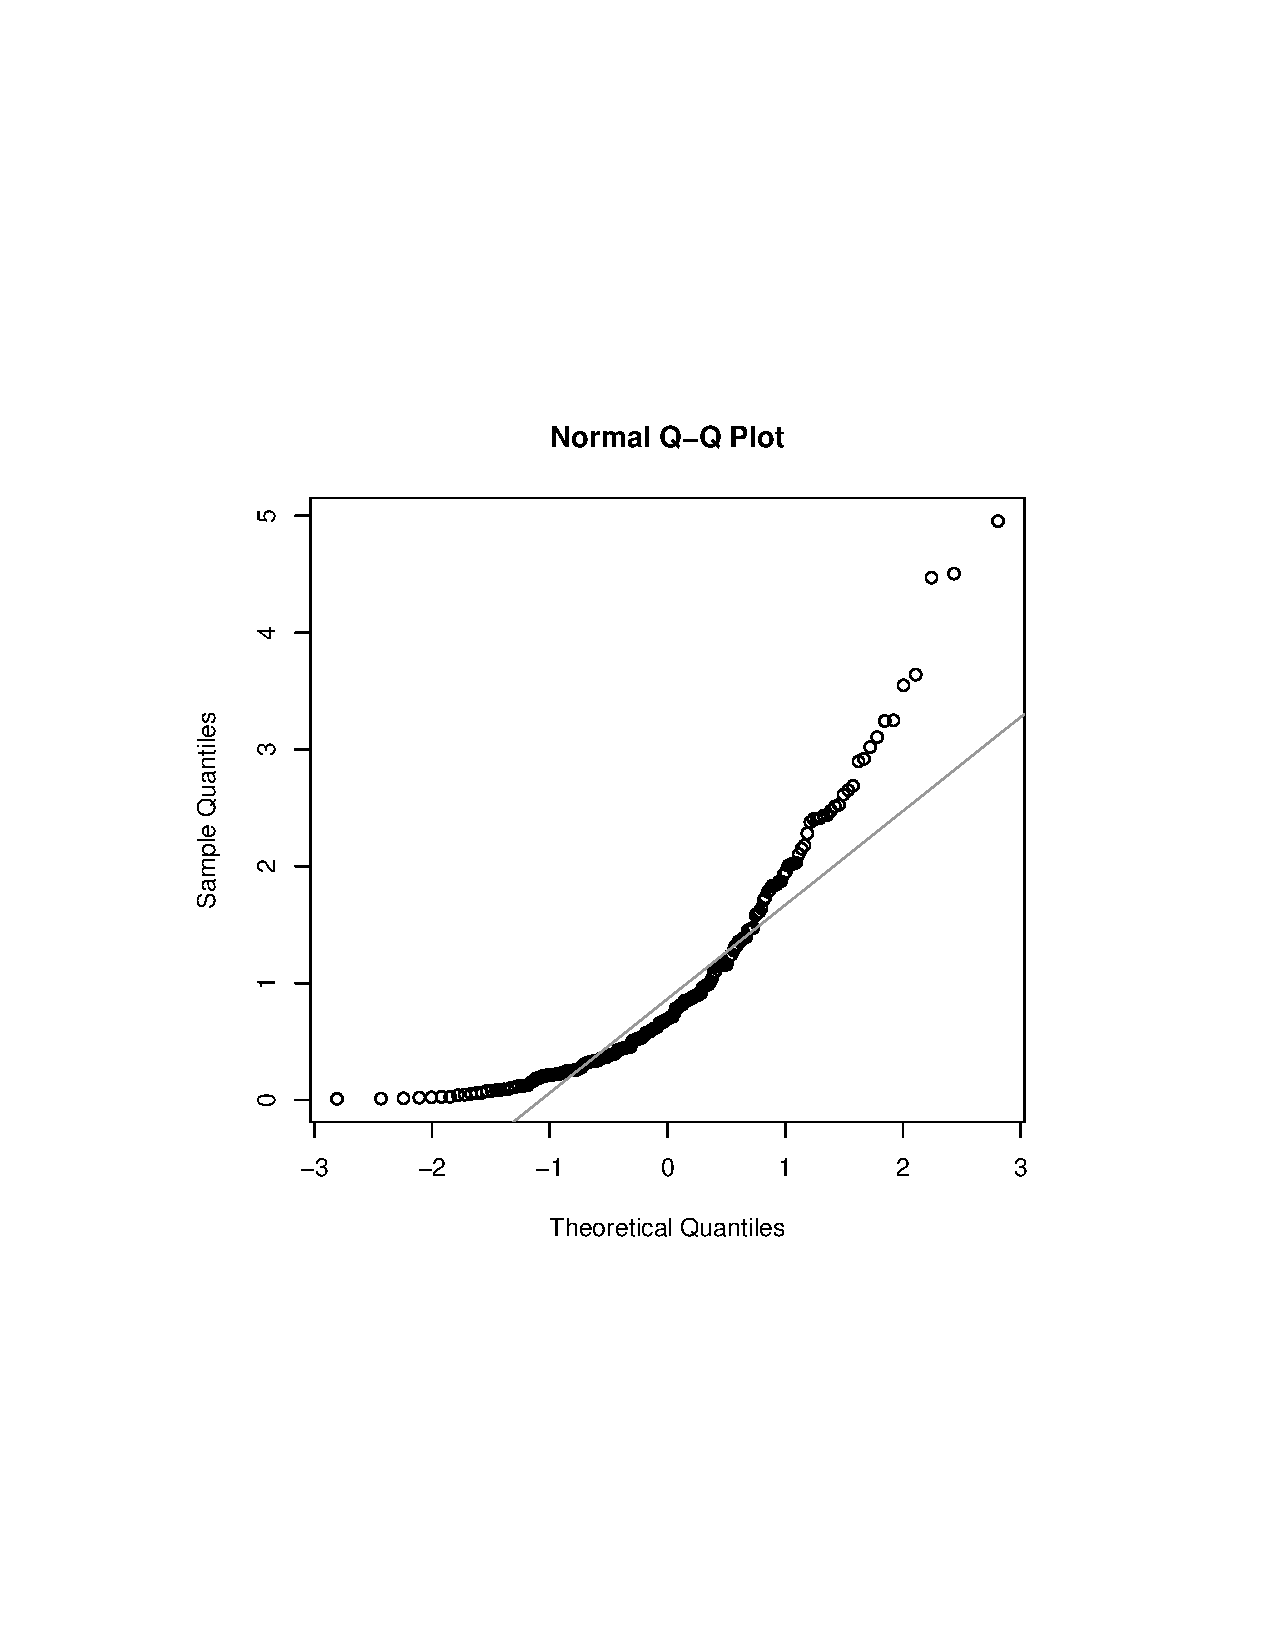
\includegraphics[width=3.5in]{qqnorm2.pdf}
\end{frame}

\begin{frame}
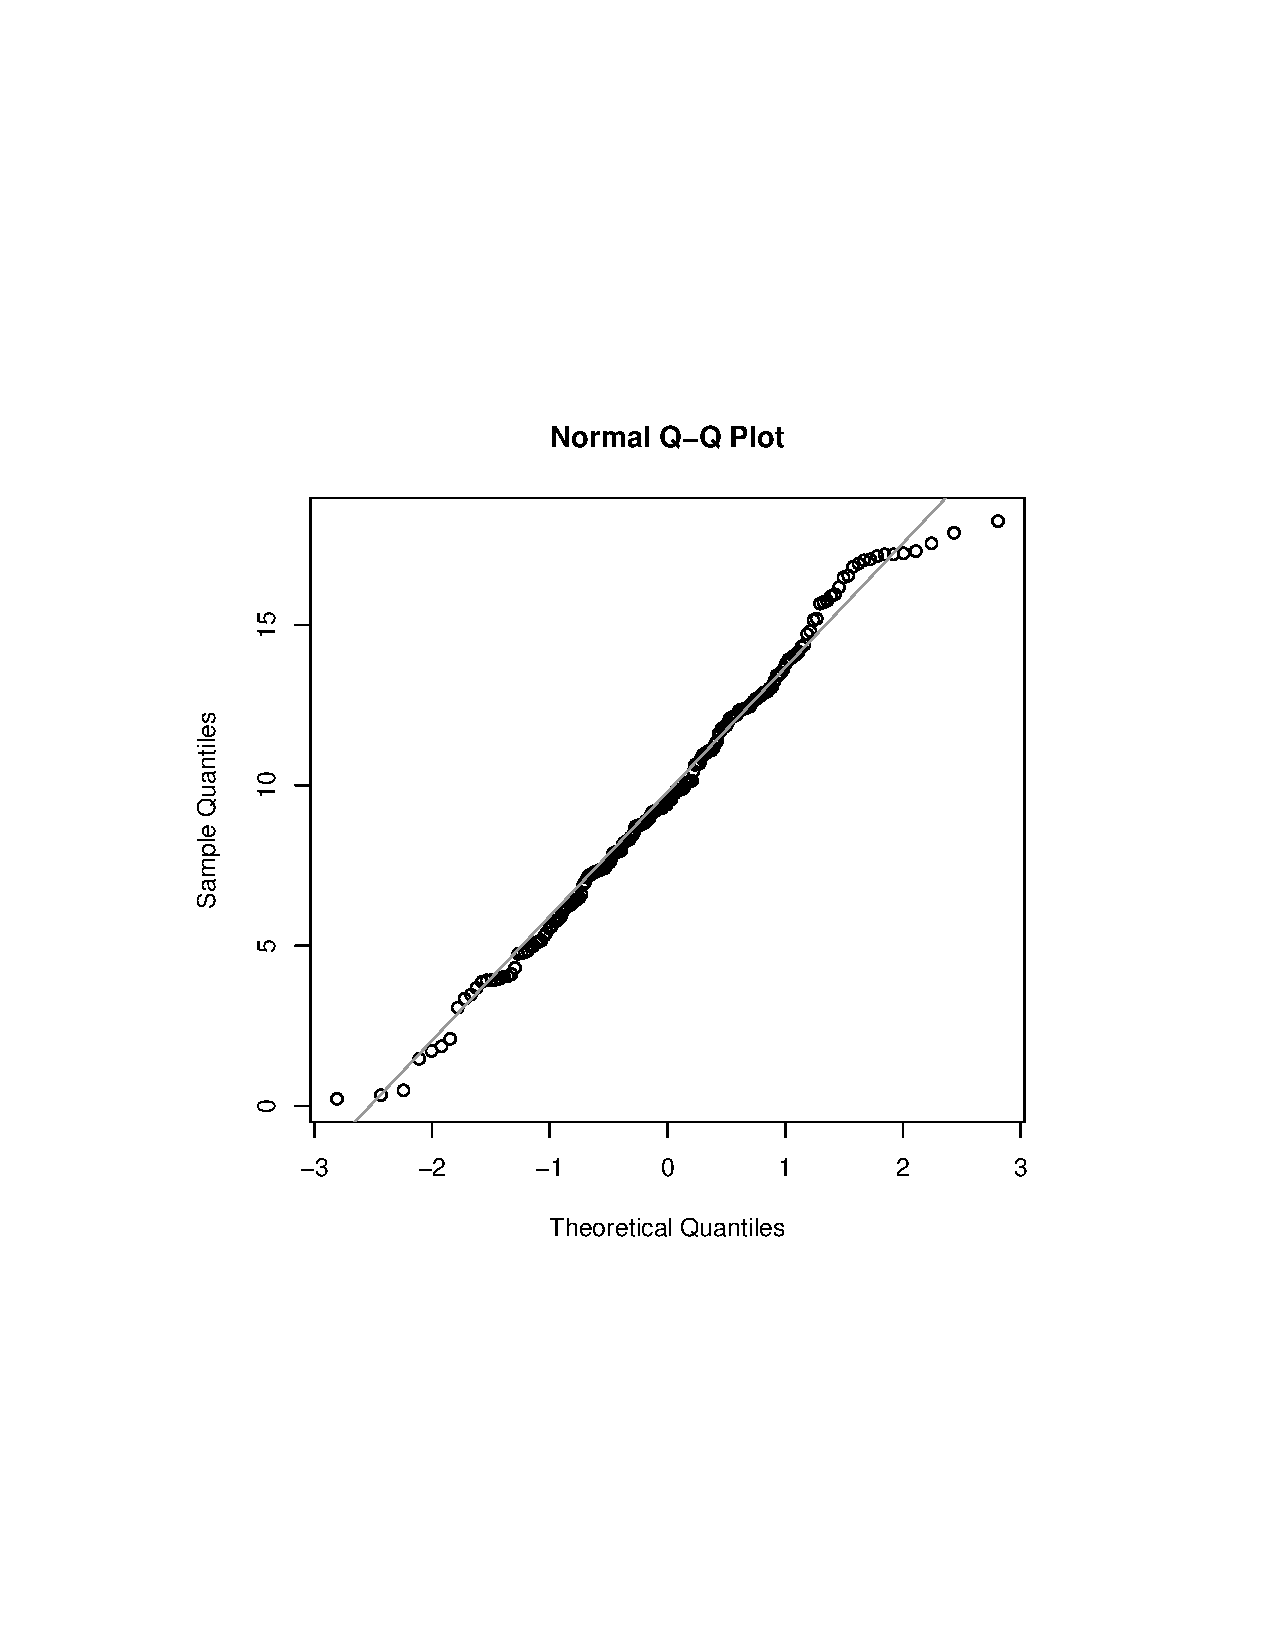
\includegraphics[width=3.5in]{qqnorm3.pdf}
\end{frame}

\section{Mosaic plots}
\begin{frame}[fragile]\frametitle{Mosaic plots}
\begin{itemize}
\item Mosaic plots are useful for displaying contingency table data
\item Consider Fisher's data regarding hair and eye color data for people from Caithness
\end{itemize}
\begin{verbatim}
library(MASS)
data(caith)
caith
mosaicplot(caith, color = topo.colors(4), 
           main = "Mosiac plot")
       fair red medium dark black
blue    326  38    241  110     3
light   688 116    584  188     4
medium  343  84    909  412    26
dark     98  48    403  681    85
\end{verbatim}
\end{frame}

\begin{frame}
  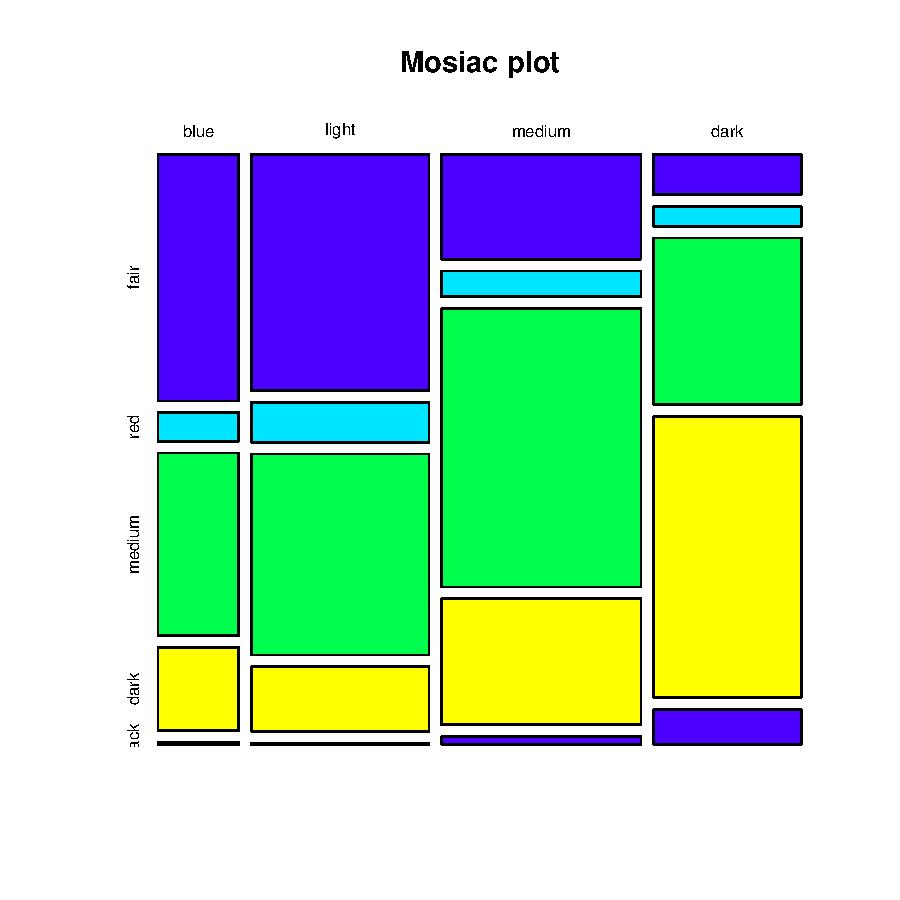
\includegraphics[width=3.5in]{mosaic.pdf}
\end{frame}

\end{document}

